\chapter{Introducción}

En este capítulo se explicará el concepto de robótica móvil\cite{RoboticaMovil}.
También se comentarán los robots submarinos, ya que en este proyecto, trataremos sobre uno de ellos, OpenROV.
Hablaremos sobre ROS (Robot Operating System), que tiene un conjunto de herramientas y atajos que facilitan la comunicación y operabilidad de los robots, ya que en uno de los capítulos del proyecto, se expondrá la integración de este framework en el ROV.
Para finalizar se describirá la estructura de la memoria y de los apartados que conlleva.

\section{Robótica móvil}
\label{cap:roboticamovil}
Generalmente las aplicaciones robóticas se centraban en los sectores manufactureros más desarrollados para la producción masiva: industria del automóvil, transformaciones metálicas, etc.

A principios de los años sesenta se introducen en la industria los robots manipuladores como un elemento más del proceso productivo. Los trabajos desarrollados por los robots manipuladores consistían frecuentemente en tareas repetitivas.

Un robot móvil puede moverse sobre entornos no estructurados, de los cuales, no se posee conocimiento. Esto lo realiza mediante la interpretación de los datos obtenidos a través de los sensores y del estado actual del vehículo. 

En general se considera que existen tres clases de robots:
\begin{itemize}
\item \textbf{Industriales}, son los de mayor difusión en tareas de alcance económico, formados por una estructura mecánica articulada, que se mueve adoptando distintas configuraciones por las órdenes recibidas de un equipo de control, generalmente, un microprocesador.
\item \textbf{Médicos}, se diseñan prótesis inteligentes para la rehabilitación de disminuidos físicos. Se procura que estas prótesis tengan la estética correspondiente a la extremidad perdida.
\item \textbf{Móviles}, tienen una plataforma mecánica dotada de un sistema de locomoción capaz de navegar a través de un determinado ambiente de trabajo.

Este tipo de robots estan dotados de un sistema de locomoción, el cual, es capaz de navegar en distintos entornos de trabajo. La locomoción puede estar diseñada con patas (equilibrio estático o dinámico) o con ruedas, que al final, son más eficientes que las piernas y son estáticamente estables. 

El mayor inconveniente de la locomoción es el desplazamiento a un lugar concreto, planificar las trayectrias y seguir la una determinada trayectoria puede resultar imposible para algunos robots.

Un robot móvil autónomo se caracteriza por una conexión inteligente entre las operaciones de percepción y actuación.
\begin{itemize}
  \item \textbf{Percepción}, es la capacidad del robot móvil para gestionar la información obtenida a través de los sensores (u otros medios) con el objetivo de lograr una navegación global o local.
   \begin{itemize}
    \item Navegación global es aquella que se apoya en mapas (SLAM). Existen varios tipos, entre los que encontramos:
      \begin{enumerate}
	\item Planificación de los caminos (planes clásicos (secuencia de subobjetivos) y planes con recursos (por donde se le recomienda ir)).
	\item Navegación basada en mapas.
	\item Listas de caminos, grafos de objetos o balizas.
	\item Grafos de visibilidad.
	\item Diagramas de Voroni.
	\item Descomposición en celdas.
	\item Planificación como descenso del gradiente.
      \end{enumerate}
    \item Navegación local es aquella que puede navegar si un mapa, y las tecnologías más usadas en ellas son:
      \begin{enumerate}
	\item Método de velocidad y curvatura (CVM), el cual, trabaja añadiendo restricciones al espacio de velocidad y escogiendo un punto del espacio que satisfaga todas las restricciones y maximice una función objetivo.
	\item Método de carriles y velocidad (LVM), esta tecnología, divide el entorno en carriles para decidir cual es el mejor camino a seguir.
	\item Método de fuerzas virturales (VFF), tanto los obstaculos como el destino ofrecen un tipo de fuerza, repulsiva y atractiva respectivamente. Al final, el movimiento del robot está gobernado por el sumatorio vectorial de dichas fuerzas.
      \end{enumerate}
   \end{itemize}
  \item \textbf{Actuación}, el robot móvil tiene que de decidir que acción es la idónea en cada momento, dependiendo del entorno y de su estado.
\end{itemize}
\end{itemize}


\section{Robots Submarinos}
\label{cap:Robots Submarinos}
En este apartado, se hará una breve introducción sobre los robots submarinos (en este trabajo nos centraremos en uno de ellos, OpenROV 2.8\footnote{https://www.openrov.com/products/openrov28/}) y donde pueden resultar de mayor utilidad.

El mundo de los robots submarinos ROV (\textit{Remote Operated Vehicle} o vehículo de operación remota) sigue creciendo año tras año. El 71\% de la superficie de la Tierra está cubierta de océanos y sin embargo, solo se ha mapeado el 5\% del suelo oceánico.

Durante los últimos años, el uso de robots submarinos ha aumentado rápidamente, ya que este vehículo puede operar en áreas más profundas y más peligrosas, a los cuales los humanos no podemos llegar. Este tipo de robot se pueden utilizar para el área de la pesca, control submarino de contaminación, manipulsación y limpieza del océano, así como de sitios nucleares.

Se trata de un área de diversas aplicaciones en el mundo real, ya que permite y facilita la exploración, estudios científicos de zonas inexploradas, la búsqueda y el rescate de navíos.

Podriamos diferenciar las diferentes áreas potenciales en las cuales tienen una aplicación como:

  \begin{itemize}
  \item \textbf{Ciencia}
    \subitem Generación de mapas del suelo marino.
    \subitem Rápida respuesta a eventos eceanográficos y geotérmicos.
    \subitem Muestreo geológico
  \item \textbf{Militar}
   \subitem Búsqueda y eliminación de minas submarinas. 
   \subitem Reconocimiento de rutas, áreas y zonas. 
   \subitem Vigilancia. 
   \subitem Búsqueda y rescate. 
   \subitem Adquisición de objetos. 
   \subitem Seguridad en las rutas. 
   \subitem Soporte en el desarrollo de la situación. 
   \subitem Soporte en la preparación del campo de batalla. 
  \item \textbf{Minería oceánica e industria del petróleo}
    \subitem Estudio del océano y evaluación de recursos.
    \subitem Construcción y mantenimiento de estructuras submarinas.
  \item \textbf{Otras}
    \subitem Inspección del casco en los barcos.
    \subitem Inspección de plantas nucleares.
    \subitem Instalación e inspección de cables. 
    \subitem Rutas turísticas bajo el mar.
    \subitem Etc.
 \end{itemize}

\begin{figure}[hbtp]
  \begin{center}
    \subfigure[Robot Deep Trekker]{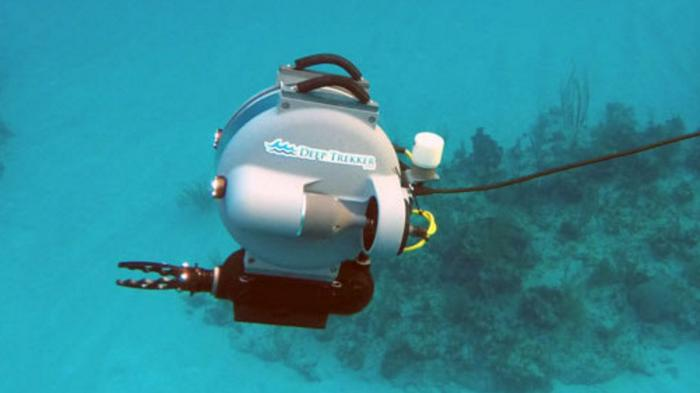
\includegraphics[width=6cm,height=5cm]{img/cap1/submarino1}}
    \subfigure[Robot OpenROV]{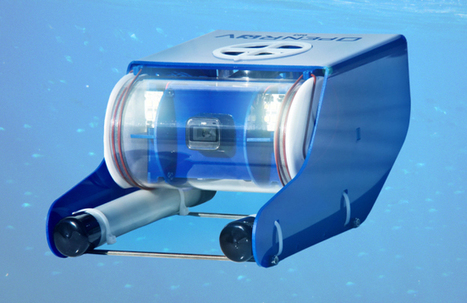
\includegraphics[width=6cm,height=5cm]{img/cap1/submarino2}}
  \end{center}
  \caption{Robots submarinos}
  \label{fig:submarino}
\end{figure}
  
\section{ROS}
\label{cap:ROS}

Sistema Operativo de Robots (en inglés \textit{Robot Operating System, ROS}\cite{ros}) es un framework para el desarrollo de software para robots. 

Implementaremos ROS en el robot submarino ya que es el framework por excelencia para el desarrollo de las aplicaciones robóticas. Contiene algoritmos implementados, además de proporcionar una arquitectura distribuida. No hace falta que los nodos de ROS interactuen en el mismo sistema ni que deban ser de la misma arquitectura, por eso es una gran ventaja utilizarlo en la tecnología de OpenROV. 

ROS provee los servicios estándar de un sistema operativo tales como abstracción del hardware, control de dispositivos de bajo nivel, implementación de funcionalidad de uso común, paso de mensajes entre procesos y mantenimiento de paquetes. Está basado en una arquitectura de grafos donde el procesamiento toma lugar en los nodos que pueden recibir, mandar y multiplexar mensajes de sensores, control, estados, planificaciones y actuadores, entre otros.

ROS tiene dos partes básicas: la parte del sistema operativo, ROS, y una suite de paquetes aportados por la contribución de usuarios que implementan la funcionalidad, como localización y mapeo simultáneo, planificación, percepción, simulación, etc.

ROS es OpenSource bajo términos de licencia BSD. Esta licencia permite libertad para uso comercial e investigador.

ROS utiliza de topics como modelo de comunicación entre procesos, a los que se les nombra como nodos. A continuación se detallan los conceptos principales de ROS:
\begin{enumerate}
 \item \textbf{Master}. Proporciona el registro de nombre. Sirve para encontrar los nodos, intercambiar mensajes e invocar servicios. 
 Para ejecutar el ROS Master, utilizaremos el comando:
  \renewcommand{\lstlistingname}{}
  \begin{lstlisting}[caption=roscore, label={lst:roscore}]
    $ roscore
  \end{lstlisting}
  
  Y se visualizará lo siguiente:
  
  \begin{figure} [hbtp]
  \begin{center}
    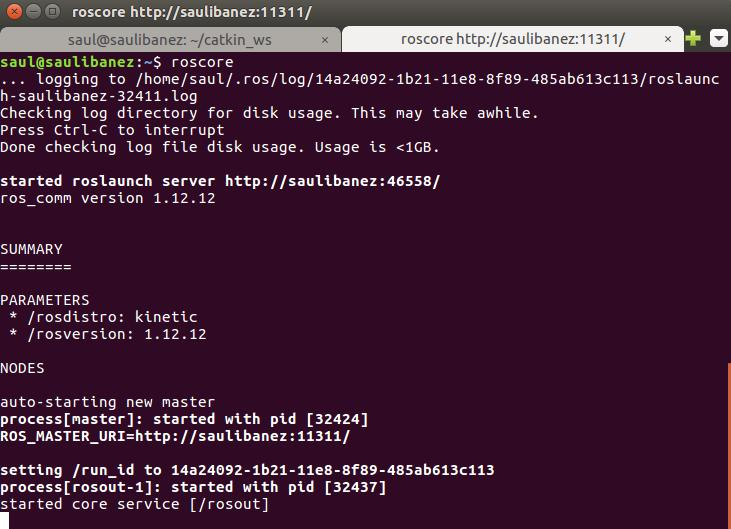
\includegraphics[width=12cm]{img/cap1/roscore}
  \end{center}
  \caption{Roscore}
  \label{fig:roscore}
  \end{figure}
  
  A partir de ahora, el sistema ya sabe donde encontrar los comandos para ejecutar ROS.
  \item \textbf{Nodos (Node)}. Son procesos de comunicación. Por ejemplo, un nodo controla la cámara, otro nodo controla los motores, etc. En general, los nodos son ejecutables que se comunican con otros procesos, a los que denominamos topics.
  \item \textbf{Mensajes}. Son estructuras de datos compuestos (integer, float, string, arrays, etc).
  \item \textbf{Topics}. Es un canal de comunicación para transmitir los datos, el cual uiliza el modo de suscriptor y publicador. Puede existir varios publicadores para un único tópico, al igual que un nodo puede publicar y/o suscribirse a múltiples topics.
  Se transimite utilizando la tecnología de TCP/IP o UDP.
\end{enumerate}


\section{Estructura de la memoria}
\label{cap:estructuradelamemoria}
En este documento se describen los aspectos más relevantes del desarrollo y montaje del robot. La memoria esta dividida en 6 capítulos. 
El primer capítulo, Introducción, se ha realizado una presentación de los robots móviles. En el segundo capítulo se define el problema y se establecen los objetivos. El montaje del robot, el entorno y las herramientas utilizadas se especifica en el tercer capítulo. En el siguiente capítulo, el cuarto, se mostrará la integración del OpenROV con ROS. En el quinto capítulo se expondrán una serie de videos comprobando el funcionamiento del OpenROV, y en el último, el sexto, expondré las conclusiones del trabajo.
